\begin{center}
 \begin{minipage}[b]{0.45\textwidth} 
\subsection*{General information}
Name: Prins David Nikolaj Vinje 
Address: Amalienborg
Zip nr. 2300 Koebenhavn S
number: 12345678
E-mail: david2300@hotmail.com
Country: Danmark
Date of birth: 11/06/1995
\newline \end{minipage}
 \hfill
\begin{minipage}[b]{3cm}
 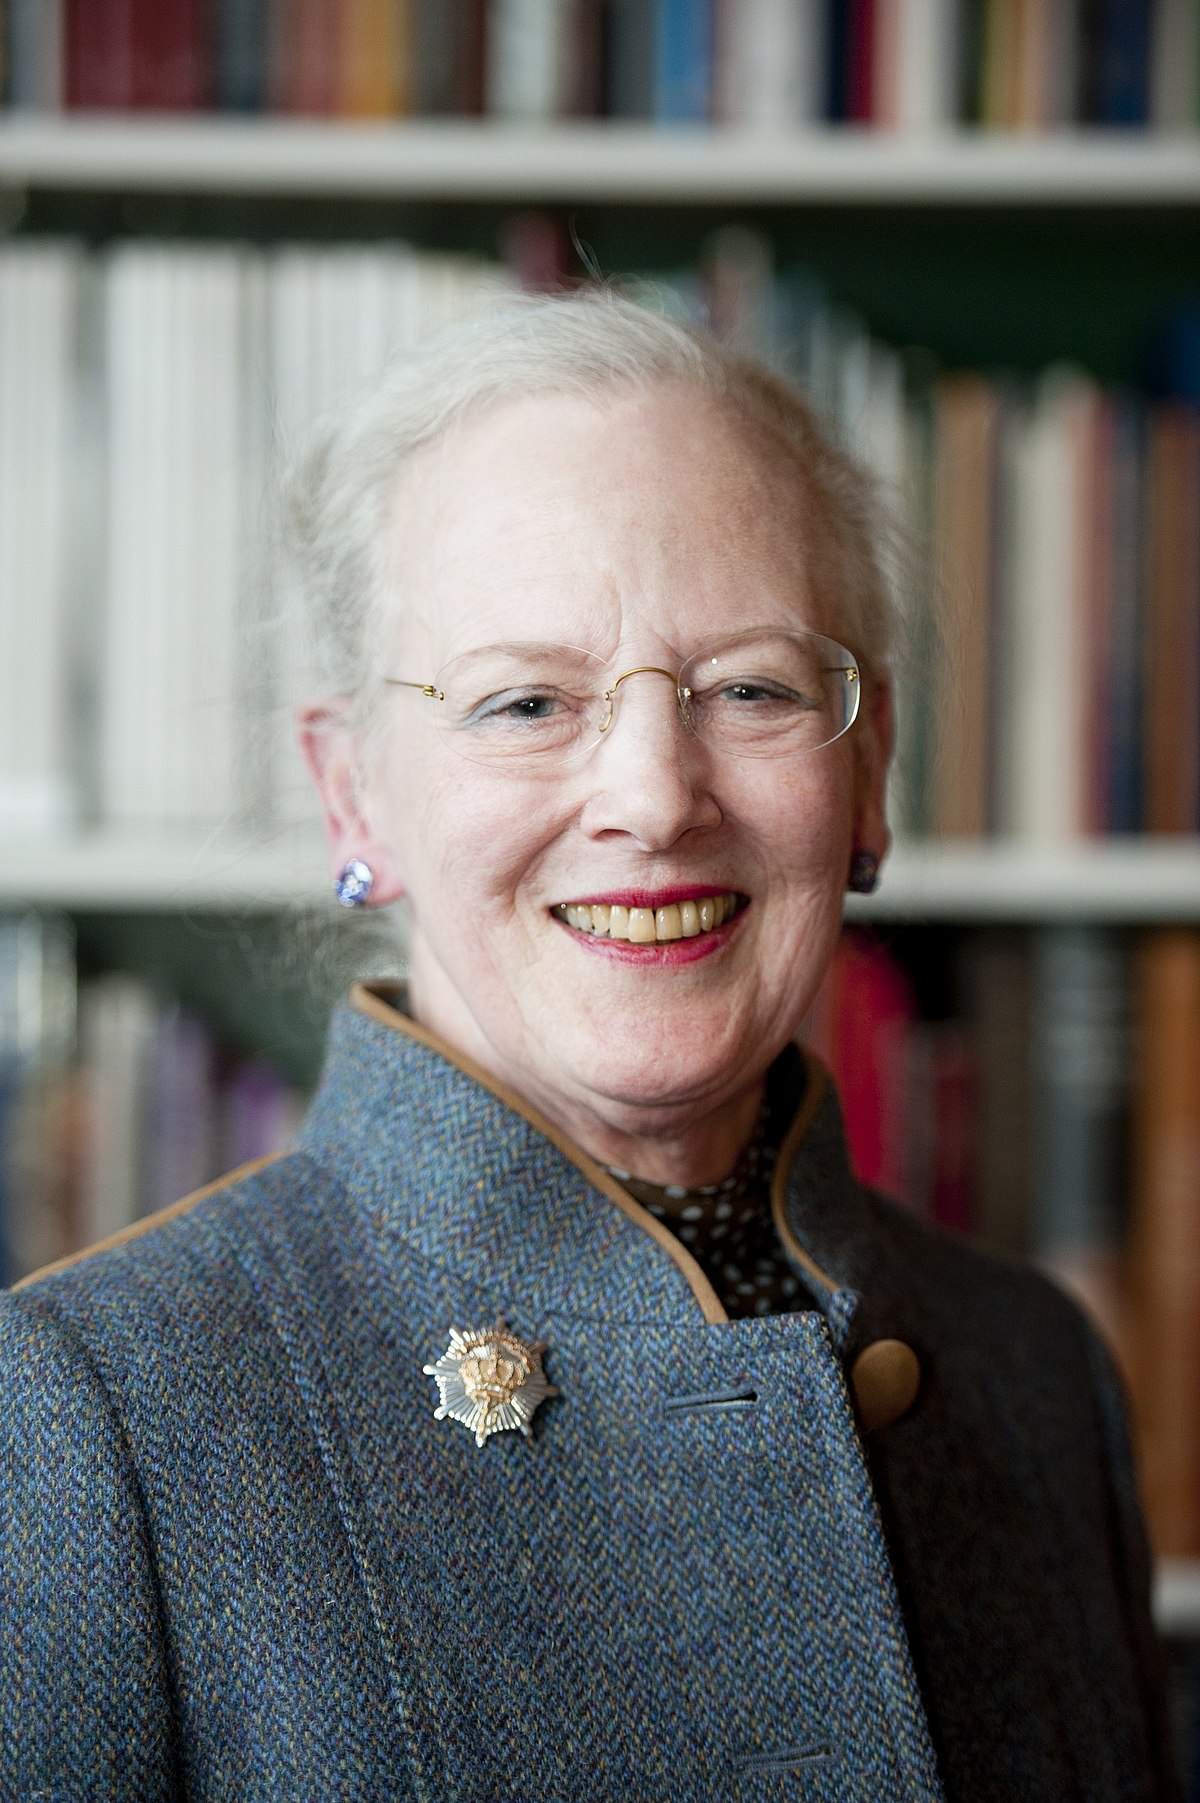
\includegraphics[height=4cm]{figures/1200px-Drottning_Margrethe_av_Danmark}
 \end{minipage}
 \end{center}

\section*{Workexperience}
\begin{itemize}
\item 2011-2012 Netto.
\item 2012-2013 Bauhaus.
\item 2013-2014 Q8
\end{itemize}
\section*{Education}
\begin{itemize}
\item 2011-2014 HTX-Hilleroed, Biotech.
\item 2015-2020 AAU Master of Software Engineering.
\end{itemize}

\section*{Free text}
Took a highschool diploma in Biotechnology and chemistry: capable of doing PCR testing.\newline highschool exam project was using c sharp (unity) to make a game.\newline currently doing a bsc in engineering (software) at Aalborg university.\newline university focuses on teamwork, so i have lots of experience with larger groups.\newline lots of skills in programming.\newline able to set up databases using SQL & net.\newline large interest in electronics. Done multiple projects.\newline capable of using machine learning using python. Also read a lot of statistics and probability theory to learn the theory behind it. Can use neural networks, to predict behavior.\newline Through my Msc i specialized in machine learning.\newline 
